%\documentclass[main.tex]{subfiles}
%\begin{document}
\section{Introduction}
\label{sec:introduction}

This report investigates an emerging paradigm for building artificial intelligence (AI) systems
based on a general class of models which we term \emph{foundation models}.\footnote{We chose the term \emph{foundation models} to capture the unfinished yet important status of these models\dash{}see \refsec{naming} for further discussion of the name.}
A foundation model is any model that is trained on broad data at scale and
can be adapted (\eg~fine-tuned) to a wide range of downstream tasks;
current examples include BERT \citep{devlin2019bert}, GPT-3 \citep{brown2020gpt3}, and CLIP \citep{radford2021learning}.
From a technological point of view,
foundation models are not new\dash{}they are based on deep neural networks and self-supervised learning,
both of which have existed for decades.
However, the sheer scale and scope of foundation models over the last few years have stretched our imagination of what is possible;
for example, GPT-3 has 175 billion parameters and
can be adapted via natural language prompts to do a passable job on a wide range
of tasks despite not being trained explicitly to do many of those tasks \citep{brown2020gpt3}.
% TODO: BERT and CLIP improve robustness 
At the same time, existing foundation models have the potential to accentuate
harms, and their characteristics are in general poorly understood.
Given their impending widespread deployment,
they have become a topic of intense scrutiny \citep{bender2021}.

%%%%%%%%%%%%%%%%%%%%%%%%%%%%%%%%%%%%%%%%%%%%%%%%%%%%%%%%%%%%
\subsection{Emergence and homogenization}

% Emergence and homogenization
The significance of foundation models can be summarized with two words: \emph{emergence} and \emph{homogenization}.
Emergence means that the behavior of a system is implicitly induced rather than explicitly constructed;
it is both the source of scientific excitement and anxiety about unanticipated consequences.
Homogenization indicates the consolidation of methodologies for building machine learning systems across a wide range of applications;
it provides strong leverage towards many tasks but also creates single points of failure. 
To better appreciate emergence and homogenization,
let us reflect on their rise in AI research over the last 30 years.

\begin{figure}[ht]
\centering
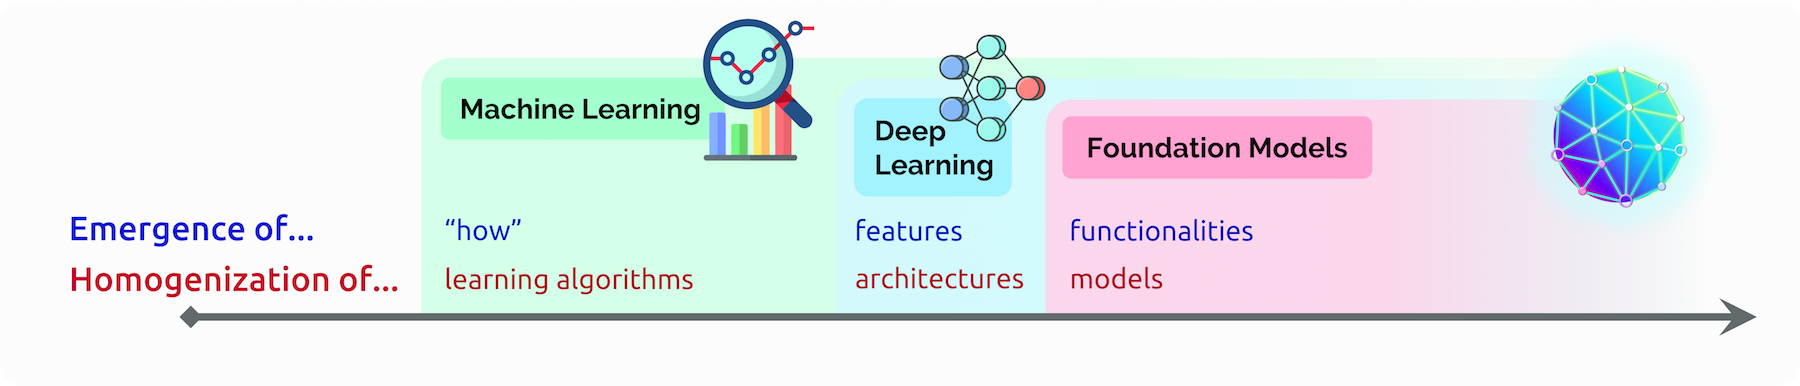
\includegraphics[width=\linewidth]{figures/Intro_Evolution.png}
\caption{
\label{fig:evolution}
The story of AI has been one of increasing \emph{emergence} and \emph{homogenization}.
With the introduction of machine learning,
\emph{how} a task is performed emerges (is inferred automatically) from examples;
with deep learning, the high-level features used for prediction emerge;
and with foundation models, even advanced functionalities such as in-context learning emerge.
At the same time,
machine learning homogenizes learning algorithms (\eg~logistic regression),
deep learning homogenizes model architectures (\eg~Convolutional Neural Networks),
and foundation models homogenizes the model itself (\eg~GPT-3).
}
\end{figure}

\paragraph{Machine learning.}

% Machine learning
Most AI systems today are powered by machine learning,
where predictive models are trained on historical data
and used to make future predictions.
The rise of machine learning within AI started in the 1990s,
representing a marked shift from the way AI systems were built previously:
rather than specifying \emph{how} to solve a task,
a learning algorithm would induce it based on data\dash{}\ie
the \emph{how} emerges from the dynamics of learning.
Machine learning also represented a step towards homogenization:
a wide range of applications
could now be powered by a single generic learning algorithm
such as logistic regression.

% Feature engineering
Despite the ubiquity of machine learning within AI,
semantically complex tasks
in natural language processing (NLP) and computer vision
such as question answering or object recognition,
where the inputs are sentences or images,
still required domain experts to perform ``feature engineering''\dash{}that is,
writing domain-specific logic to convert raw data into higher-level features
(\eg SIFT \citep{lowe1999sift} in computer vision)
that were more suitable for popular machine learning methods.

\paragraph{Deep learning.}

% Deep learning
Around 2010, a revival of deep neural networks
under the moniker of \emph{deep learning} \citep{lecun2015deep} started gaining traction in the field of machine learning.
Deep learning was fueled by larger datasets,
more computation (notably, the availability of GPUs),
and greater audacity.
Deep neural networks would be trained on the raw inputs (\eg pixels),
and higher-level features would emerge through training.
This led to massive performance gains on standard benchmarks,
for example, in the seminal work of AlexNet \citep{krizhevsky2012imagenet} on the ImageNet dataset \citep{deng2009imagenet}.
Deep learning also reflected a further shift towards homogenization:
rather than having bespoke feature engineering pipelines for each application,
the same deep neural network architecture could be
used for many applications.

\paragraph{Foundation models.}

Foundation models have taken shape most strongly in NLP, so we focus our story there for the moment.
By the end of 2018, the field of NLP was about to undergo another seismic change,
marking the beginning of the era of foundation models.
On a technical level, foundation models are enabled by
\emph{transfer learning} \citep{thrun1998lifelong} and \emph{scale}.
The idea of transfer learning is to take the ``knowledge'' learned from one task (\eg object recognition in images)
and apply it to another task (\eg activity recognition in videos).
Within deep learning, \emph{pretraining} is the dominant approach to transfer learning:
a model is trained on a surrogate task (often just as a means to an end) and then adapted to
the downstream task of interest via \emph{fine-tuning}.

% Scale: hardware + Transformer + data
Transfer learning is what makes foundation models possible,
but scale is what makes them powerful.
Scale required three ingredients:
(i) improvements in computer \emph{hardware}\dash{}\eg~GPU throughput and memory have increased 10$\times$ over the last four years (\refsec{systems});
(ii) the development of the Transformer model architecture \citep{vaswani2017attention}
that leverages the parallelism of the hardware to train much more expressive models than before (\refsec{modeling});
and (iii) the availability of much more training data.

% pretraining based on annotated data
The importance of the availability of data and the ability to harness it cannot be underestimated.
Transfer learning with annotated datasets has been common practice for at least a decade,
for example, pretraining on the ImageNet dataset \citep{deng2009imagenet} for image classification
in the computer vision community.
However, the non-trivial cost of annotation imposes a practical limit on the benefits of pretraining.  

% Self-supervised learning
In \emph{self-supervised learning} on the other hand,
the pretraining task is derived automatically from unannotated data.\footnote{
Interestingly, self-supervised learning
was dominant in the early days of deep learning
\citep{hinton2006fast},
but was for a decade largely overtaken by pure supervised learning as labeled datasets became larger.}
For example, the masked language modeling task used to train BERT \citep{devlin2019bert} is to
predict a missing word in a sentence given its surrounding context (\eg~\emph{I like \rule{1cm}{0.15mm} sprouts}).
Self-supervised tasks are not only more scalable, only depending on unlabeled data,
but they are designed to force the model to predict parts of the inputs, 
making them richer and potentially more useful than models trained on a more limited label space.

% Self-supervised learning in NLP
There had been considerable progress in self-supervised learning dating back to word embeddings
\citep{turian2010word,mikolov2013efficient,pennington2014glove},
which associated each word with a context-independent vector,
provided the basis for a wide range of NLP models.
Shortly thereafter, self-supervised learning based on autoregressive language modeling
(predict the next word given the previous words) \citep{dai2015semi}
became popular.
This produced models that represented words in context, such as
GPT \citep{radford2018improving},
ELMo \citep{peters2018elmo},
and ULMFiT \citep{howard2018universal}.\footnote{The prescient work of \citet{collobert2008unified}
is related: they trained on a scalable task akin to masked language modeling jointly with downstream tasks,
rather than producing a single foundation model that can be adapted after the fact to downstream tasks.}

The next wave of developments in self-supervised learning\dash{}BERT \citep{devlin2019bert}
GPT-2 \citep{radford2019language},
RoBERTa \citep{liu2019roberta},
T5 \citep{raffel2019exploring},
BART \citep{lewis2020bart}\dash{}quickly followed,
embracing the Transformer architecture,
incorporating more powerful deep bidirectional encoders of sentences,
and scaling up to larger models and datasets.

% Foundation models: sociological development
While one can view this last wave of technical developments purely through the lens of self-supervised learning,
there was a sociological inflection point around the introduction of BERT.
Before 2019, self-supervised learning with language models was essentially a \emph{subarea} in NLP,
which progressed in parallel to other developments in NLP.
After 2019, self-supervised learning with language models became more of a \emph{substrate} of NLP,
as using BERT has become the norm.
The acceptance that a single model could be useful for such a wide range of tasks
marks the beginning of the era of foundation models.

% Homogenization in NLP
Foundation models have led to an unprecedented level of \emph{homogenization}:
Almost all state-of-the-art NLP models
are now adapted from one of a few foundation models,
such as BERT, RoBERTa, BART, T5, etc.
While this homogenization produces extremely high leverage
(any improvements in the foundation models can lead to immediate benefits
across all of NLP), it is also a liability; all AI systems might
inherit the same problematic biases of a few foundation models \citep[][\textit{inter alia}]{bolukbasi2016, caliskan2017, abid2021})\dash{}see \refsecs{fairness}{ethics} for further discussion.

We are also beginning to see a homogenization across research communities.
For example, similar Transformer-based sequence modeling approaches
are now applied to text \citep{devlin2019bert, radford2019language, raffel2019exploring},
images \citep{visual_transformer, chen2020imagegpt}, speech \citep{Liu2020MockingjayUS}, tabular data
\citep{Yin2020TaBERTPF},
protein sequences \citep{rives2021},
organic molecules \citep{rothchild2021c5t5},
and reinforcement learning \citep{Chen2021DecisionTR, Janner2021ReinforcementLA}.
These examples point to a possible future where we have
a unified set of tools for developing foundation models across a wide range of modalities \citep{Tamkin2021DABS}.

\begin{figure}[t]
\centering
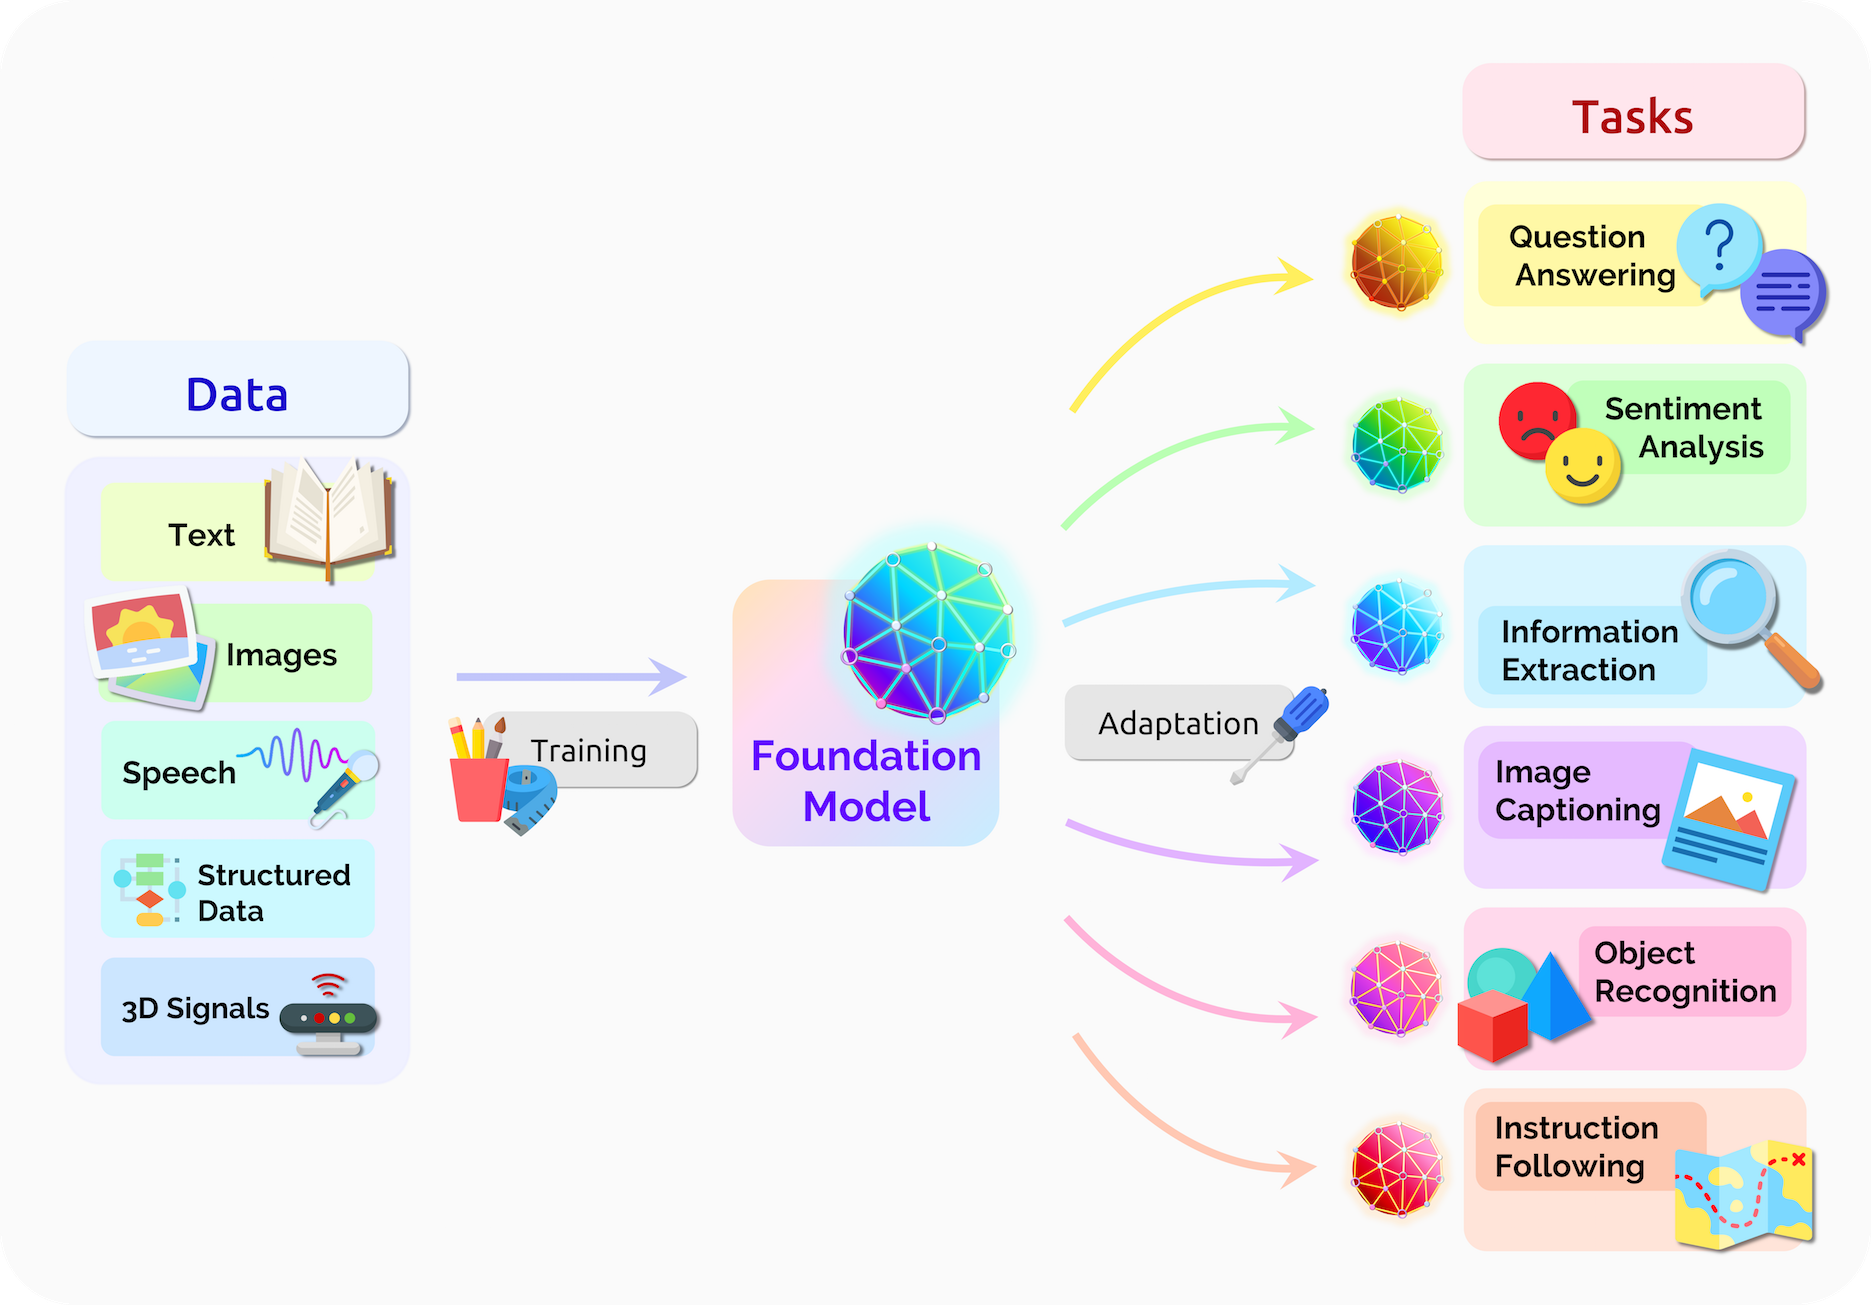
\includegraphics[width=\linewidth]{figures/Intro_Framework.png}
\caption{
\label{fig:framework}
A foundation model can centralize the information from all the data from various modalities.
This one model can then be adapted to a wide range of downstream tasks.
}
\end{figure}

% Multimodal
Besides the homogenization of approaches,
we also see the homogenization of actual models across research communities in the form of \emph{multimodal models}\dash{}\eg{}foundation models trained on language and vision data
\citep{luo2020univl,kim2021vilt,cho2021unifying,ramesh2021zeroshot,radford2021learning}.
Data is naturally multimodal in some domains---\eg~medical images, structured data, clinical text in healthcare (\refsec{healthcare}).
Thus, multimodal foundation models are a natural way of fusing all the relevant information about a domain,
and adapting to tasks that also span multiple modes (\reffig{framework}).

% GPT-3, emergence
Foundation models have also led to surprising emergence which results from scale.
For example, GPT-3 \citep{brown2020gpt3}, with 175 billion parameters compared to GPT-2's 1.5 billion,
permits \emph{in-context learning}, in which the language model can be adapted to a downstream task simply by
providing it with a \emph{prompt} (a natural language description of the task),
an emergent property that was neither specifically trained for nor anticipated to arise.

%%%%%%%%%%%%%%%%%%%%%%%%%%%%%%%%%%%%%%%%%%%%%%%%%%%%%%%%%%%%

% Homogenization and emergence interact badly
Homogenization and emergence interact in a potentially unsettling way.
Homogenization could potentially provide enormous gains for many
domains where task-specific data is quite limited\dash{}see the  opportunities presented in several such domains (\eg~\refsec{healthcare}, \refsec{law}, \refsec{education});
on the other hand, any flaws in the model are blindly inherited by all adapted models (\refsec{fairness}, \refsec{ethics}).
Since the power of foundation models comes from their \emph{emergent qualities}
rather than their explicit construction,
existing foundation models are hard to understand (\refsec{evaluation}, \refsec{theory}, \refsec{interpretability})
and they have unexpected failure modes (\refsec{security}, \refsec{robustness}).
Since \emph{emergence} generates substantial uncertainty over the capabilities and flaws of foundation models,
aggressive homogenization through these models is risky business.
Derisking is the central challenge in the further development of foundation models
from an ethical (\refsec{ethics}) and AI safety (\refsec{ai-safety}) perspective.

\subsubsection{Naming.}
\label{sec:naming}

We introduce the term \textit{foundation models} to fill a void in describing the paradigm shift we are witnessing; we briefly recount some of our reasoning for this decision.
Existing terms (\eg \emph{pretrained model}, \emph{self-supervised model}) partially capture the technical dimension of these models,
but fail to capture the significance of the paradigm shift in an accessible manner for those beyond machine learning.
\emph{Language model} is too narrow; as we describe, the scope of foundation models goes well beyond language.
We also considered terms such as \emph{general-purpose model} and \emph{multi-purpose model} that capture the important aspect that these models can serve multiple downstream tasks,
but both fail to capture their unfinished character and the need for adaptation.
Terms such as \emph{task-agnostic model} would capture the manner of training, but fail to capture the significant implication to downstream applications.

We chose the new term \emph{foundation models} to identify the models and the emerging paradigm that are the subject of this report.
In particular, the word ``foundation'' specifies the role these models play:
a foundation model is itself incomplete but serves as the common basis from which many task-specific models are built via adaptation.
We also chose the term ``foundation" to connote the significance of architectural stability, safety, and security:
poorly-constructed foundations are a recipe for disaster and well-executed foundations are a reliable bedrock for future applications.
At present, we emphasize that we do not fully understand the nature or quality of the foundation that foundation models provide; we cannot characterize whether the foundation is trustworthy or not.
Thus, this is a critical problem for researchers, foundation model providers, application developers who rely on foundation models, policymakers, and society at large to address.

%%%%%%%%%%%%%%%%%%%%%%%%%%%%%%%%%%%%%%%%%%%%%%%%%%%%%%%%%%%%
\subsection{Social impact and the foundation models ecosystem}
\label{sec:ecosystem}

\begin{figure}[t]
\centering
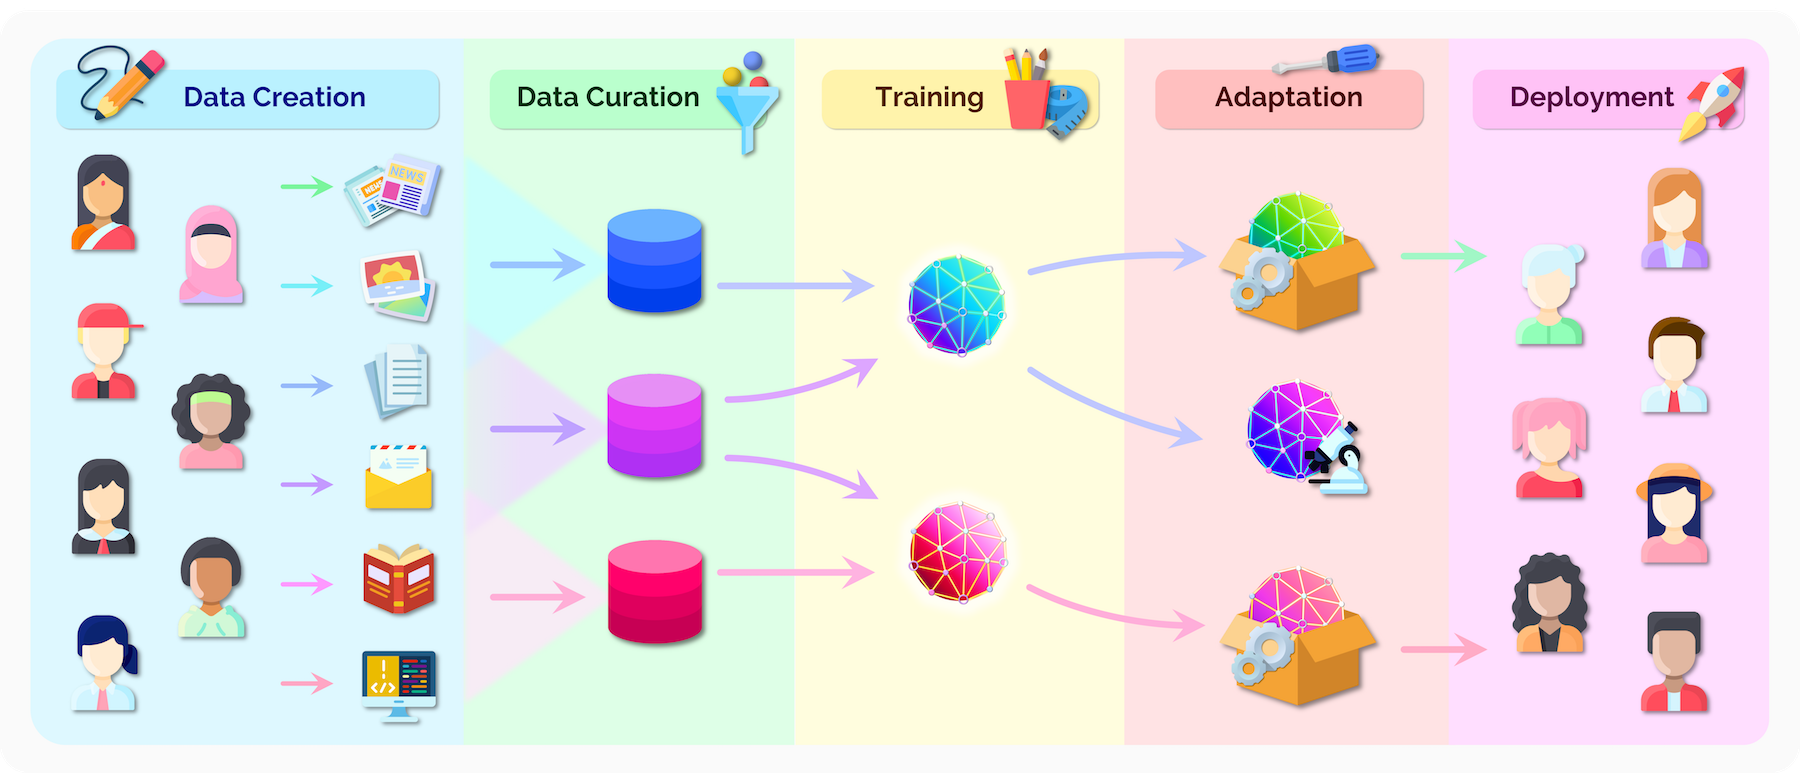
\includegraphics[width=\linewidth]{figures/Intro_Ecosystem.png}
\caption{
\label{fig:ecosystem}
Before reasoning about the social impact of foundation models,
it is important to understand that they are part of a broader ecosystem
that stretches from data creation to deployment.
At both ends, we highlight the role of people as the ultimate source of data into training of a foundation model,
but also as the downstream recipients of any benefits and harms.
Thoughtful data curation and adaptation should be part of the responsible development of any AI system.
Finally, note that the deployment of adapted foundation models is a decision separate from their construction,
which could be for research.
}
\end{figure}

% Lots of examples
Foundation models are scientifically interesting due to their impressive performance and capabilities, 
but what makes them critical to study is the fact that they are quickly being integrated into real-world deployments of AI systems with far-reaching consequences on people.
For example, Google search, which boasts 4 billion users,
now depends on foundation models like BERT \citep{devlin2019bert} as one of its
signals.\footnote{https://blog.google/products/search/search-language-understanding-bert/}

% Types of impact
We must thus pause and ask:
What is the nature of this social impact?
In this report, we address many aspects of this question:
the potential exacerbation of social inequities (\refsec{fairness}),
the economic impact due to increased capabilities (\refsec{economics}),
the environmental impact due to increased computation demands (\refsec{environment}),
potential concerns of amplifying disinformation (\refsec{misuse}),
legal ramifications due to powerful generative capabilities (\refsec{legality}),
ethical issues resulting from homogenization,
and the broader political economy in which foundation models are developed and deployed (\refsec{ethics}).
Given the protean nature of foundation models and their unmapped capabilities,
how can we responsibly anticipate and address the ethical and societal considerations they raise?
A recurring theme is that it is easier
to reason about the social impact of specific systems deployed to specific users
than it is to reason about the social impact of foundation models,
which could be adapted to any number of unforeseen downstream systems.

% Ecosystem
Before attempting to answer these questions,
we need to lay some groundwork.
First, let us distinguish between \emph{research} on foundation models and \emph{deployment} of foundation models.
Most of what is publicly known is foundation models research\dash{}through academic papers,
demonstrations, and progress on leaderboards.
While the production of knowledge can play a vital role in shaping the future,
the direct social impact is through the actual deployment of these models,
which is governed by proprietary practices on often private data.
Sometimes the deployment is through new products\dash{}\eg~GitHub's
Copilot\footnote{https://copilot.github.com/} based on OpenAI's Codex model
\citep{chen2021evaluating}, but often,
it is through upgrades to existing products (\eg~Google search using BERT).
Research models are often not extensively tested and might have unknown failure modes;
warning labels should be placed on research models that are not fit to deploy.
On the other hand, deployed foundation models that actually affect people's lives
should be subject to much more rigorous testing and auditing.

% Deployment
To further understand the research and deployment of foundation models,
we must zoom out and consider the full \emph{ecosystem} that these foundation models inhabit,
from data creation to actual deployment.
It is important to note that the foundation model is only one component (though
an increasingly important component) of an AI system.
Simplifying, we can think about the ecosystem of a foundation model in terms of
sequence of stages, extending the training and adaptation stages from before.\footnote{In practice, the end of the pipeline is followed by monitoring, and feedback is
used to readjust the previous stages.}
Appropriately, as we're interested in social impact,
\emph{people} occupy both ends of the pipeline.
This ecosystem view allows us to see that different questions about foundation models
(\eg~whether a foundation model is ethical) should actually be answered with respect to different stages.
\begin{enumerate}
  \item \textbf{Data creation}:
    Data creation is fundamentally a human-centric process:
    all data is created by people and most data is at least implicitly about people.
    Sometimes data is created by people for other people in the form of emails, articles, photos, etc.,
    and sometimes it is a measurement of people (\eg~genomic data)
    or a measurement of the environment people live in (\eg~satellite images).
    It is important to note that all data has an owner and is created with a purpose
     (where that purpose may or may not include training a foundation model).

  \item \textbf{Data curation}:
    Data is then curated into datasets.
    There is no single natural distribution of data;
    even the most permissive Internet crawl requires some selection and post-filtering.
    Ensuring data relevance and quality while respecting legal and ethical constraints is critical but challenging.
    While this is recognized in industry, it is underappreciated in AI research (\refsec{data}).

  \item \textbf{Training}:
    Training foundation models on these curated datasets\footnote{A foundation model (\eg~Codex) can also be trained with another
    model (\eg~GPT-3) as a starting point.}
    is the celebrated centerpiece in AI research,
    though it is only one of many stages.

  \item \textbf{Adaptation}:
    In the context of machine learning research,
    adaptation is about creating a new model based on the foundation model
    that performs some task (\eg~document summarization).
    For deployment, adaptation is about creating a system,
    which requires potentially many different modules, custom rules
    (\eg~restrictions on the output space) or classifiers (\eg~for toxicity
    classification),
    and combination with other complementary signals (\eg~a question answering
    model's generated answers would be validated against relevant documents).
    For example, a problematic model capable of generating toxic content might be tolerable
    if appropriate precautions are taken downstream.
    The extra application-specific logic is crucial for mitigating harms.

  \item \textbf{Deployment}:
    The direct social impact of an AI system occurs when it is deployed to people.
    Though we would not want to deploy potentially harmful foundation models trained on questionable data,
    there might still be value in permitting them in research to advance scientific understanding,
    though one must still exercise caution.
    More generally, it is standard practice in large-scale deployments
    to conduct gradual releases, where deployment happens to an increasing fraction of users;
    this can partially mitigate any potential harms.
\end{enumerate}

% Every stage of the pipeline
While this report is about foundation models,
it is important to note that many of the impacts come from decisions made in
other stages in the pipeline,
and thoughtful monitoring and intervention is needed at every stage.
While large organizations might own the entire pipeline,
each stage could be performed by a different organization,
\eg~a company which specializes in creating custom foundation models for
various domains that application-developers can use.

\paragraph{Think ecosystem, act model.}
While the social impact depends on the whole ecosystem,
it is still important to be able to reason about the social implications of a foundation model,
given that many researchers' and practitioners' purview is restricted to the training stage.
This is difficult because foundation models are unfinished intermediate
objects that can be adapted to many downstream applications, sometimes by an
entirely different entity for unforeseen purposes.
What we need are two things:
(i) surrogate metrics for a representative set of potential downstream evaluation (\refsec{evaluation}),
and (ii) a commitment to documenting these metrics \citep{Mitchell_2019}
similar to data sheets for materials such as metals and plastics,
which can be adapted to many downstream use cases.

Characterizing the potential downstream social impact of foundation models
is challenging and demands a deep understanding of both the technological ecosystem
and of society.
One cannot fully assess the harms (\refsec{fairness}) of a foundation model without recognizing how it will be deployed,
and one cannot just define automatic metrics without considering the rich social and historical context.

%%%%%%%%%%%%%%%%%%%%%%%%%%%%%%%%%%%%%%%%%%%%%%%%%%%%%%%%%%%%
\subsection{The future of foundation models}
\label{sec:developers}

Foundation models have demonstrated raw potential,
but we are still in the early days.
Despite their deployment into the real world,
these models are very much research prototypes that are poorly understood.
Even the professional norms\dash{}what Robert Merton calls the ethos of science \citep{merton1979normative}\dash{}around foundation models are underdeveloped.
For example, there is lack of agreement on basic questions such as when models are ``safe'' to release
or how the community should react in response to methodological misconduct.
Given that the future of foundation models is thus filled with uncertainty,
a big question is: who will determine this future?

\paragraph{Disciplinary diversity.}

% Technology in academia+industry, foundation models in industry
The technology behind foundation models is based on decades of research in
machine learning, optimization, NLP, computer vision, and other fields.
These technical contributions have come from both academia and industrial research labs.
However, research on building foundation models themselves has occurred almost exclusively in industry\dash{}big tech
companies such as Google, Facebook, Microsoft, or Huawei, or startups such as
OpenAI or AI21 Labs, though AI2 is a notable exception \citep{peters2018elmo,zellers2019neuralfakenews}.

% What we need to do, academia can do it
The furious pace of technological progress and the entrenchment due to centralization
raise powerful concerns that demand the attention of humanists and social scientists in addition to technologists.
We should not rely on post-hoc audits of ethical and social consequences,
conducted only after the technical architecture and deployment decisions have been made.
We instead need to infuse social considerations and ethical design
deeply into the technological development of foundation models and
their surrounding ecosystem from the start.
Academic institutions are unique in that they host the widest set of disciplines under one roof,
thus bringing together computer scientists, social scientists, economists, ethicists, legal scholars, etc.
Given the importance of disciplinary diversity in understanding and solving problems that combine technical, ethical, legal, social, and political dimensions \citep{hong2004groups,solomon2006norms,steel2018multiple},
we therefore see academia as playing a crucial role
in developing foundation models in such a way to promote their social benefit and mitigate their social harms,
as well as determining the contexts under which actions in each of the stages of the ecosystem (\refsec{ecosystem}) ranging from data curation to deployment should be strictly prohibited.

\paragraph{Incentives.}

% Industry aligns somewhat, but differ from social benefit
The political economy in which foundations models are designed, developed, and deployed provides an inevitable incentive structure for decision-making at every stage. How people and institutions respond to incentives is an elementary lesson of economics.
Market-driven commercial incentives can align well with social benefit:
making foundation models more accurate, reliable, safe, and efficient while searching for a wide variety of potential use cases
can produce a great deal of social utility.
However, commercial incentives can also lead to market failures and underinvestment in domains where shareholders are unable to capture the value of innovation. 
Just as the pharmaceutical industry has little incentive to devote significant resources to the research and development of malaria treatments, because poor people cannot afford medications,\footnote{See https://www.gatesfoundation.org/about/our-role.} the tech industry has little incentive to devote significant resources to technologies designed for improving the condition of poor and marginalized people \citep{reich2021system}. What's more, the commercial incentive can lead companies to ignore social externalities \citep{acemoglu2021redesigning, reich2021system} such as the technological displacement of labor, the health of an informational ecosystem required for democracy, the environmental cost of computing resources, and the profit-driven sale of technologies to non-democratic regimes.
Finally, there is little incentive for any given company to create
an open, decentralized ecosystem for developing foundation models
that encourages broad participation.

% Universities capture social value
In contrast,
the long-standing and deeply-seated research mission of universities is the
production and dissemination of knowledge and creation of global public goods \citep{kerr2001university,rhoten2011knowledge,nussbaum2010not}. 
We believe that academia is distinctively positioned to
shape the development of foundation models to ensure that we capture
directions with potentially large social benefit that might not otherwise be prioritized by industry.

\paragraph{Loss in accessibility.}

% Deep learning was open
Unfortunately, academia has not been able to participate in the fullest way possible
due to the loss in accessibility.
One of the often overlooked effects of the deep learning revolution
was the increase in reproducibility and open science:
it increasingly became the norm to publicly release code and datasets, and
packages such as TensorFlow \citep{abadi2016tensorflow} and PyTorch
\citep{paszke2019pytorch} made it much easier for people to collaborate and
build off of each other’s work. 
Initiatives like the ML Reproducibility
Challenge\footnote{https://paperswithcode.com/rc2020} as well as
reproducibility checklists adopted by major conferences
\citep{pineau2020improving}, alongside platforms like CodaLab 
Worksheets\footnote{https://worksheets.codalab.org/} helped advance community
standards for reproducibility.
This resulted in a surge in technological innovation and progress.

% Foundation models are becoming more closed
Foundation models start to roll back this positive trend.
Some models (\eg{}GPT-3) are not released at all (only API access to a limited pool of people).
Even datasets (\eg{}for GPT-2) are not released.
While trained models may be available (\eg{}BERT),
the actual training of foundation models is
unavailable to the vast majority of AI researchers,
due to the much higher computational cost and the complex engineering requirements.

% Emergence demands larger scale
Some meaningful research can still be done by training smaller models within reach of an academic budget,
and indeed the surprisingly regularity predicted by scaling laws \citep{kaplan2020} make this a viable strategy
for cases where the differences due to scale are quantitative (\eg~accuracy goes up).
However, due to the emergent nature of these foundation models,
some functionalities like in-context learning have only been demonstrated in models of sufficient size,
so scale is needed to even ask the right questions.

% Using released model isn't enough
It is also possible to productively study pre-existing models that have been released; indeed, this has
led to a large subcommunity within NLP for probing these models \citep{rogers2020primer, manning2020emergent}.
Having access to existing models can be useful for powering downstream applications or identifying defects (\eg{}bias),
but this might not be enough for us to design better architectures or training objectives for foundation models
that can fix these defects (\eg{}mitigate the bias).
It is worth reflecting on how much of NLP research today is based on BERT,
a particular (and somewhat arbitrary) foundation model.
Given the need to infuse social awareness and ethical design into the construction of these models,
it is possible that we need to build foundation models that look quite different from what exists today.
This will demand intense experimentation at scale.

% Barrier of entry rising (even will hurt startups)
Community efforts such as EleutherAI\footnote{https://www.eleuther.ai/} and Hugging Face's BigScience project\footnote{https://bigscience.huggingface.co/}
are attempting to train large foundation models,
but the gap between the private models that industry can train
and the ones that are open to the community will likely remain large if not grow.
Further, today startups (OpenAI, Anthropic, AI21 Labs, etc.) are much more well-resourced than academia
and can therefore still afford to train the largest foundation models (\eg~OpenAI's GPT-3).
However, big tech companies are on a completely different level
in terms of resources, especially in terms of the infrastructure, users, and data that come from their market position.
The fundamental centralizing nature of foundation models
means that the barrier to entry for developing them will continue to rise,
so that even startups, despite their agility, will find it difficult to compete,
a trend that is reflected in the development of search engines \citep{radinsky2015data}.

% Public infrastructure
One way to close the resource gap is for the government to invest in public infrastructure.
We can look to Big Science projects such as the Hubble Space Telescope and the Large Hadron Collider as inspiration,
where substantial investment made possible fundamental scientific discoveries which wouldn't have been possible.
One can imagine a similar infrastructure for computing, from which academic research on foundation models would greatly benefit.
In the US, the nascent National Research Cloud initiative\footnote{https://hai.stanford.edu/policy/national-research-cloud} is a step in this direction.

% Massive decentralized
Another complementary approach is to rely on volunteer computing,
in which any of the billions of computing devices (nodes) can connect to a central server and contribute computation.
The Folding@home project has successfully implemented this approach for simulating protein dynamics \citep{beberg2009folding}.
Recently, the Learning@home project is attempting to harness volunteer computing for training foundation models
\citep{Ryabinin2020Learninghome}.
The high latency connections between nodes and the high bandwidth requirements for training foundation models
make this an open technical challenge.

\paragraph{Summary.}
% Summary
There are tremendous economic incentives to push the capabilities and scale of foundation models,
so we anticipate steady technological progress over the coming years.
But the suitability of a technology relying largely on emergent behavior
for widespread deployment to people is unclear.
What is clear that we need to be cautious,
and that now is the time to establish the professional norms that will enable the responsible research and deployment
of foundation models.
Academia and industry need to collaborate on this:
industry ultimately makes concrete decisions about how foundation models will be deployed,
but we should also lean on academia,
with its disciplinary diversity and non-commercial incentives around knowledge production and social benefit,
to provide distinctive guidance on the development and deployment of foundation models
that is both technically and ethically grounded.

%%%%%%%%%%%%%%%%%%%%%%%%%%%%%%%%%%%%%%%%%%%%%%%%%%%%%%%%%%%%
\subsection{Overview of this report}
\label{sec:overview}

\begin{figure}[t]
\centering
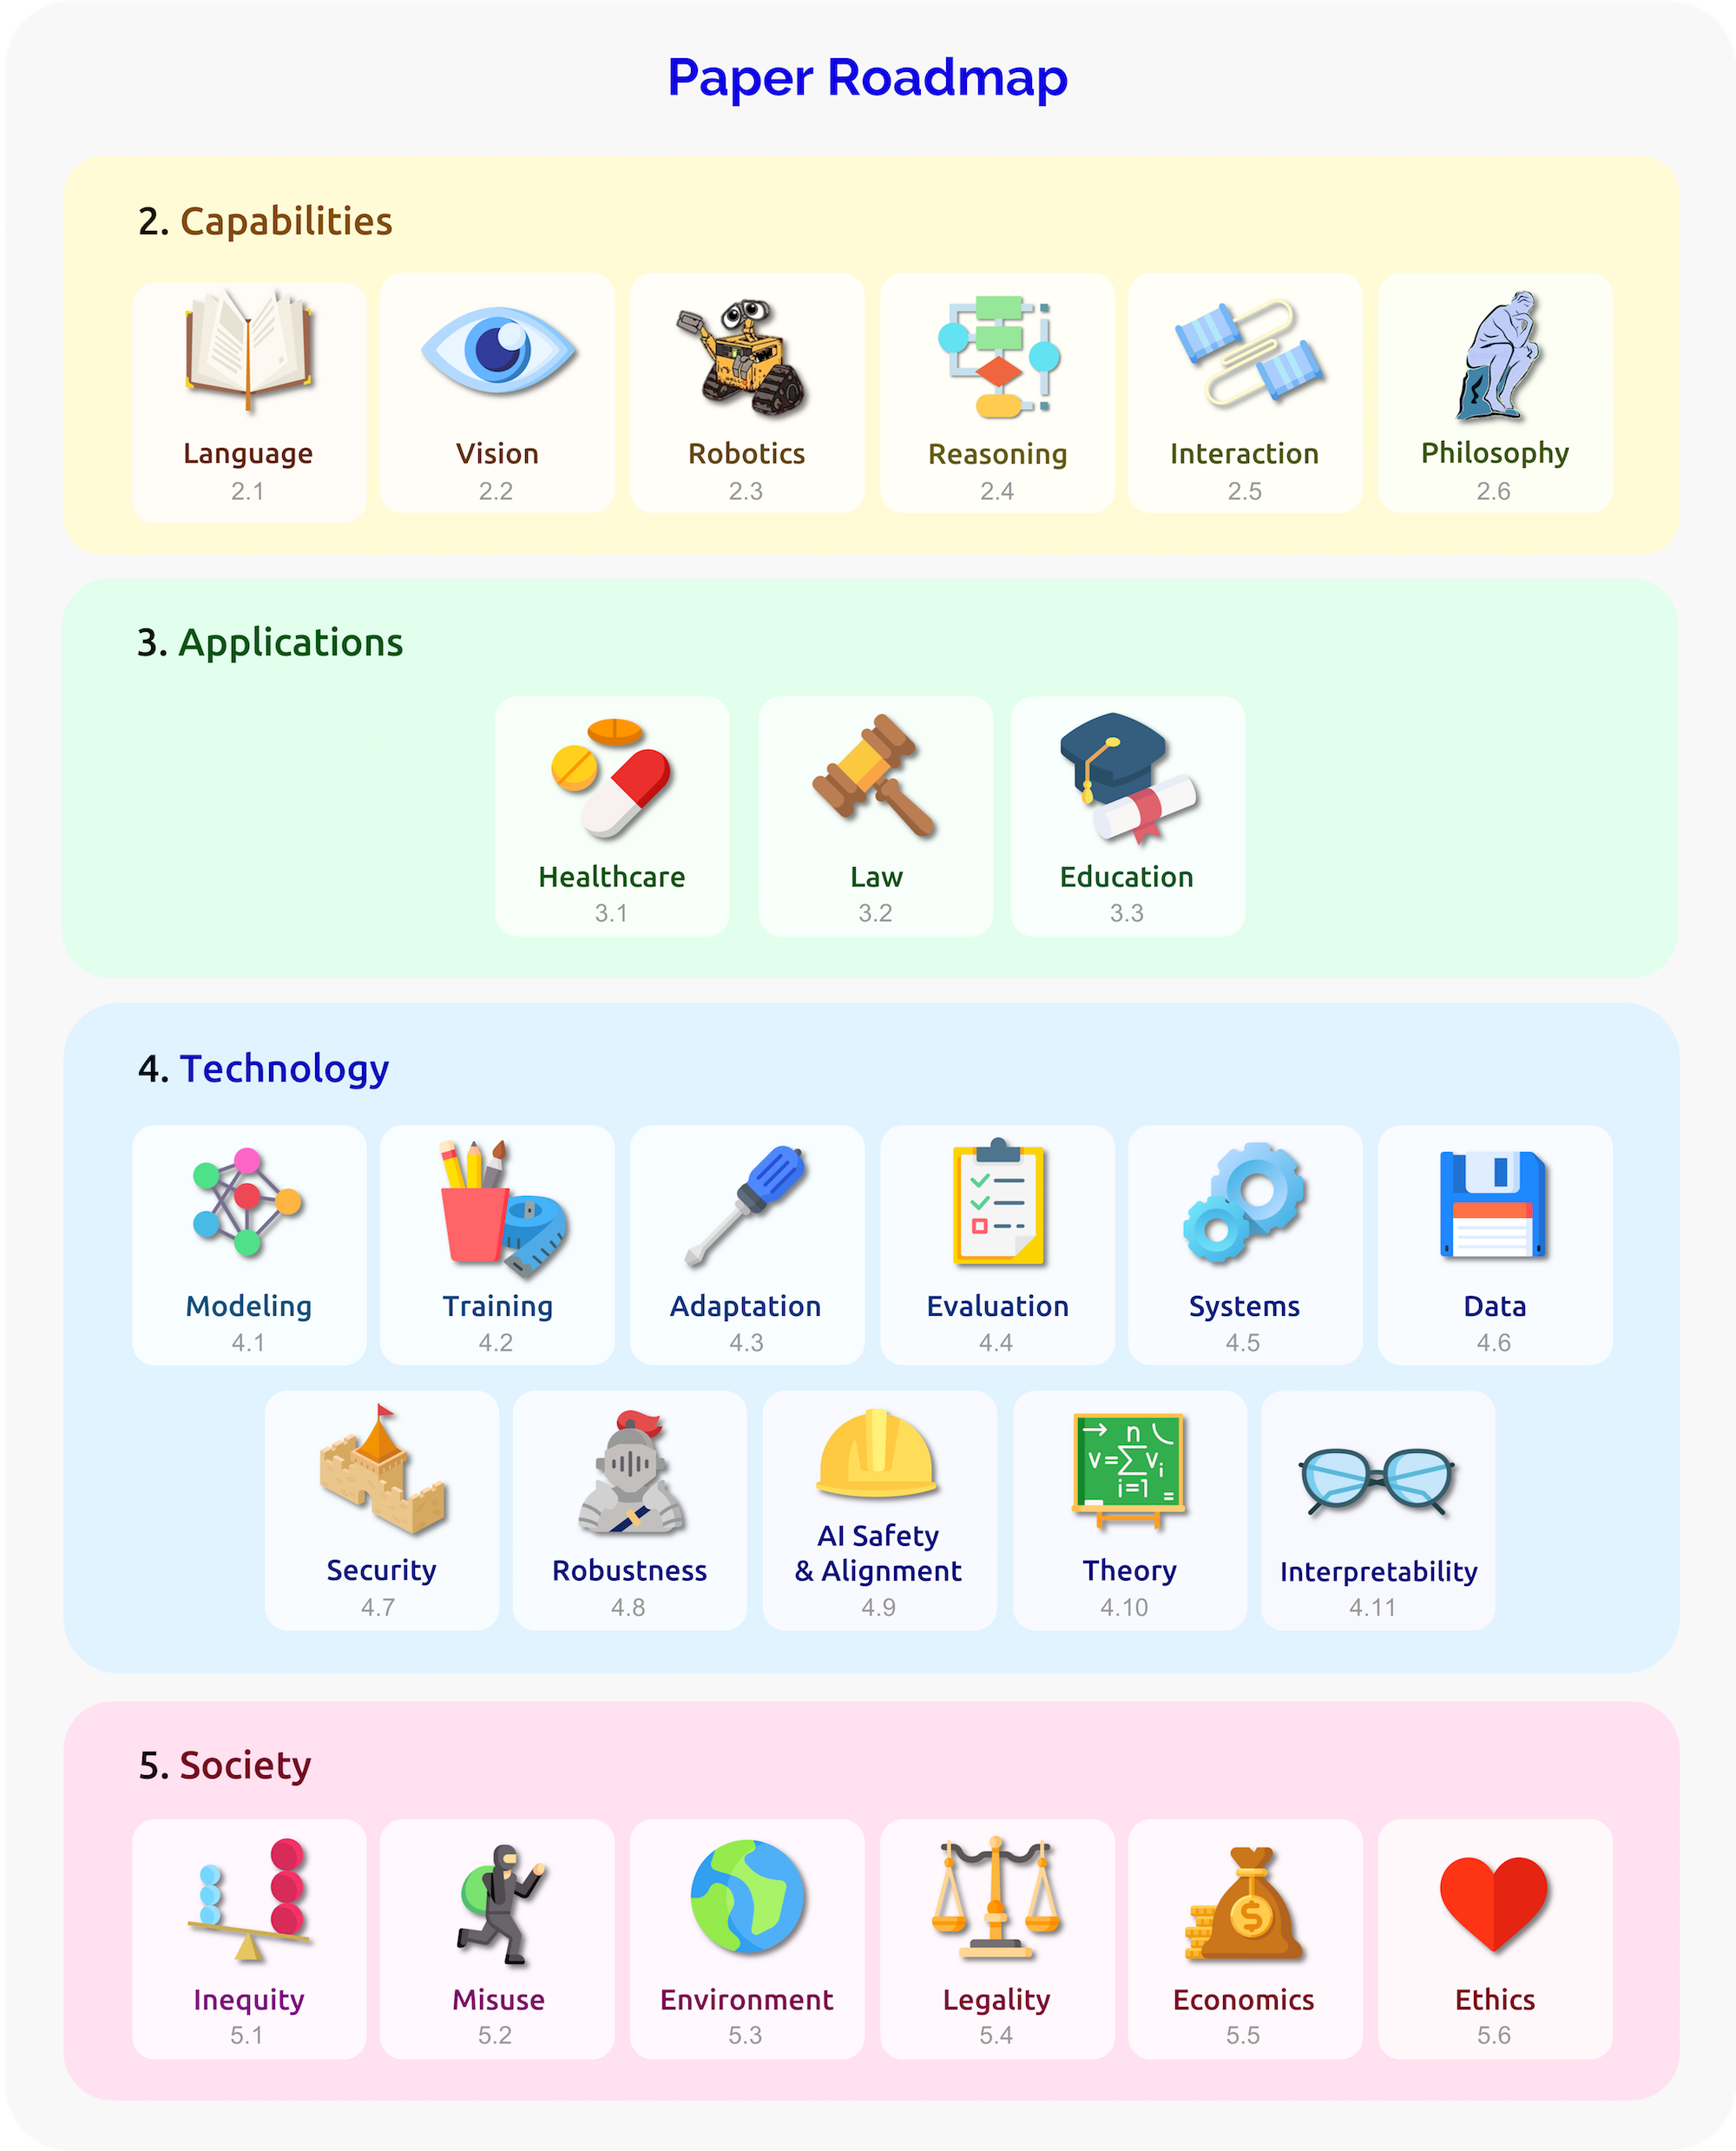
\includegraphics[width=\linewidth]{figures/Roadmap.png}
\caption{This report is divided into four parts: capabilities, applications, technology, and society,
where each part contains a set of sections,
and each section covers one aspect of foundation models.
\label{fig:roadmap}
}
\end{figure}

In March 2021, we created an informal community at Stanford University of students, faculty, and researchers
interested in some aspect of foundation models.\footnote{This community
led to the founding of the \emph{Center for Research on Foundation Models (CRFM)},
a new interdisciplinary initiative at the Stanford Institute for Human-Centered AI (HAI).}
From the very beginning, the community included not just AI researchers,
but those eager to apply foundation models to their domain (\eg{}healthcare and law),
as well as those who were interested in societal concerns (\eg{}ethics and economics).
As discussions progressed,
we noticed that there were many gaps in mutual understanding\dash{}how the
technology worked, how industry develops foundation models, how to think about the ethical
concerns, etc.,
and existing literature only covered bits and pieces.
We wanted to therefore provide a fuller picture of foundation models, identify
opportunities and risks, and establish a constructive vision for the future responsible development of foundation models.

The writing of this report was an experiment:
we had over 100 people from different backgrounds come together to write
single report covering a wide range of aspects of foundation models.
A large part of this report is a survey of existing work, but through many discussions,
we have unified it in one report to highlight all the interdisciplinary connections.

\paragraph{Structure.}

% This report
The report is divided into 26 sections, each discussing one aspect of foundation models.
The sections are grouped into four parts:
capabilities (\refsec{capabilities}),
applications (\refsec{applications}),
technology (\refsec{technology}),
and society (\refsec{society}),
although there are many connections across sections.
These connections highlight an integrated approach
in which the technologies and capabilities are developed in a way that is sensitive to
real societal concerns, while being inspired by and grounded out in applications.

% Incomplete
While we have sought to capture most of the important topics surrounding
foundation models, this report will inevitably be incomplete,
especially as the field evolves quickly.
For example, many applications (\eg~natural sciences, music, finance, agriculture) are not included,
though they are as likely to be affected as the applications we have chosen to discuss.
It would also be interesting to study how foundation models relate to research in neuroscience, cognitive science, and psychology to explain intelligence and aid efforts in computational social science to understand society.

\paragraph{Author contributions.}

Percy Liang initiated and conceptualized the framing and structure of the overall report.
He and Rishi Bommasani worked together to lead the decentralized writing effort
and provided guidance on individual sections.
Drew A. Hudson created all the figures in the report, discussing
their structure and content with the authors of each section.
Each of the 26 sections of this report was written
by a subset of authors, whose names are listed at the beginning of each section.
There were, however, many discussions that spanned multiple sections,
so the actual contributions to each section generally came from a broader set.
Finally, we note that not all the views expressed in this report are held
by all the authors.

\subsubsection{Overview of capabilities}

Foundation models possess various \emph{capabilities} that applications can draw from.
We have chosen to discuss five potential capabilities:
the ability to process different modalities (\eg language, vision), to affect
the physical world (robotics), to perform reasoning, and to interact with
humans (interaction).  Finally, we conclude with a philosophical discussion of potential limits on their capabilities.

\paragraph{\hyperref[sec:language]{§\ref{sec:language}:~Language.}}

NLP as a field has blazed the trail for foundation models.
While these models dominate standard benchmarks, there is a clear gap between the capabilities these models acquire currently and those that characterize language as a complex system for human communication and thought.
To understand this rift, we emphasize the full range of \textit{linguistic variation} (\eg~different styles, dialects, languages), which poses an opportunity and challenge given some variants are data-limited.
Further, child \textit{language acquisition} is more sample efficient than the training of foundation models; we examine how signals beyond text and grounding may help to bridge this gap.
Both of these characteristics of language provide clear directions for future foundation models research.

\paragraph{\hyperref[sec:vision]{§\ref{sec:vision}:~Vision.}}
Computer vision led the adoption of deep learning in AI \cite{russakovsky2015imagenet}, demonstrating that pretraining models on large-scale annotated datasets can transfer to numerous downstream settings.
Now, pretraining on web-scale raw data instead of curated datasets, foundation models are on the rise in computer vision~\citep[\eg][]{radford2021learning}.
These models have shown promising results for standard tasks in the field, like image classification and object detection, and training on \textit{multimodal and embodied} data beyond images may enable progress on significant challenges (\eg~3D geometric and physical understanding, commonsense reasoning).
We also discuss some of the key challenges in modeling (\eg~the ability to scale effectively to videos) and evaluation (\eg~the measurement of higher-order capabilities) along with the applications (\eg~ambient intelligence for healthcare) and societal considerations (\eg~surveillance) that will determine the impact of foundation models for computer vision going forward.

\paragraph{\hyperref[sec:robotics]{§\ref{sec:robotics}:~Robotics.}}

A longstanding goal of robotics research is to develop ``generalist'' robots capable of performing myriad tasks across physically diverse environments.
Unlike language and vision, which have led the way with foundation models both due to the abundance of raw data to train these models on and the availability of virtual applications to apply these models to, robotics faces fundamental challenges due to being anchored to the physical world.
The principal challenge for robotics to leverage foundation models is acquiring \textit{sufficient data} of the \textit{right form} that is conducive to learning: we explore how plentiful data (\eg~generic videos of humans, amongst others) that is not specific to particular environments and across modalities (\eg~language, vision) may help to bridge this gap.
If foundation models work well in robotic contexts, this allows for the easier \textit{specification and learning of tasks} by robotic agents, ushering in new applications (\eg~household tasks) and heightening the importance of \textit{robustness and safety} (\eg~formal safety evaluation).

\paragraph{\hyperref[sec:reasoning]{§\ref{sec:reasoning}:~Reasoning and search.}}

Reasoning and search problems such as theorem proving and program synthesis have been long-standing challenges in AI. The combinatorial search space renders traditional search-based methods intractable.
However, humans are known to operate intuitively even in the most mathematical of domains~\citep{LakoffNunez00},
and indeed existing work such as AlphaGo have already shown that deep neural networks can be effective in guiding the search space.
But humans also transfer knowledge across tasks, facilitating
much more efficient adaptation and the ability to reason more abstractly.  Foundation models offer the possibility of closing this gap: their multi-purpose nature along with their strong generative and multimodal capabilities offer new leverage for controlling the combinatorial explosion inherent to search.

\paragraph{\hyperref[sec:interaction]{§\ref{sec:interaction}:~Interaction.}}
Foundation models show clear potential to transform the developer and user experience for AI systems: foundation models lower the difficulty threshold for \textit{prototyping and building} AI applications due to their sample efficiency in adaptation, and raise the ceiling for \textit{novel user interaction} due to their multimodal and generative capabilities.
This provides a synergy we encourage going forward: developers can provide applications that better fit the \textit{user's needs and values}, while introducing far more dynamic forms of interaction and opportunities for \textit{feedback}.

\paragraph{\hyperref[sec:philosophy]{§\ref{sec:philosophy}:~Philosophy of understanding.}}

What could a foundation model come to understand about the data it is trained on? Focusing on the case of natural language, we identify different positions on the nature of understanding and explore their relevance for our central question. Our tentative conclusion is that skepticism about the capacity of future foundation models to understand natural language may be premature, especially where the models are trained on multi-modal data.

%%%%%%%%%%%%%%%%%%%%%%%%%%%%%%%%%%%%%%%%%%%%%%%%%%%%%%%%%%%%
\subsubsection{Overview of applications}
At present, foundation model research is largely confined to computer science and AI, with the impact of foundation models and the applications they support largely being centered in the tech industry.
Moving forward, foundation models present clear potential to transform and extend the reach of AI across many sectors beyond the tech industry, suggesting a more pervasive effect on people's lives.
While there is a multitude of applications and domains to consider, we we have chosen three applications \dash{} healthcare, law, and education \dash{} because they represent foundational pillars of our society.  
For foundation models to significantly contribute to these application domains, models will require specific capabilities (\refsec{capabilities}) as well as technical innovation (\refsec{technology}) to account for the unique considerations in each domain.
Further, since these domains are critical to societal function (\refsec{society}), applying foundation models in these domains requires engaging with deeply sociotechnical matters such as those those pertaining to data (\refsec{data}), privacy (\refsec{security}), interpretability (\refsec{interpretability}),  fairness (\refsec{fairness}) and ethics (\refsec{ethics}).

\paragraph{\hyperref[sec:healthcare]{§\ref{sec:healthcare}:~Healthcare and biomedicine.}}

Healthcare tasks (\eg~patient care via disease treatment) and biomedical research (\eg~scientific discovery of new therapies) require expert knowledge that is limited and expensive. 
Foundation models present clear opportunities in these domains due to the \textit{abundance of data} across \textit{many modalities} (\eg~images, text, molecules) to train foundation models, as well as the value of improved sample efficiency in adaptation due to the cost of expert time and knowledge. 
Further, foundation models may allow for improved \textit{interface design} (\refsec{interaction}) for both healthcare providers and patients to interact with AI systems, and their generative capabilities suggest potential for \textit{open-ended research problems} like drug discovery. 
Simultaneously, they come with clear risks (\eg~exacerbating historical biases in medical datasets and trials). 
To responsibly unlock this potential requires engaging deeply with the sociotechnical matters of data sources and privacy as well as model interpretability and explainability, alongside effective regulation of the use of foundation models for both healthcare and biomedicine.

\paragraph{\hyperref[sec:law]{§\ref{sec:law}:~Law.}}

Legal applications require that attorneys read and produce long coherent
narratives that incorporate shifting contexts and decipher ambiguous legal standards.
Foundation models may provide benefits in this domain: \textit{ample data} exists in the form of legal documents and their generative capabilities are well-suited to the \textit{many generative tasks required in law}, but significant improvements are required for foundation models to be able to reliably \textit{reason over various sources} of information to generate \textit{truthful} long-form documents.
As is the care in healthcare (\refsec{healthcare}), the sample efficiency of adaptation for foundation models is of heightened value given the costs of expert time and knowledge in the legal domain, which may allow for the \textit{re-allocation of expertise} towards pressing problems of justice and government service.
The responsible development of foundation models for law will require specific consideration of privacy, and highlights core limitations of existing foundational models that will require fundamental advances with respect to \textit{provenance} for their behavior and \textit{guarantees} for the factuality of their generation.

\paragraph{\hyperref[sec:education]{§\ref{sec:education}:~Education.}} 

Education is a complex and subtle domain; effective teaching involves reasoning about student cognition and should reflect the learning goals of students.
The nature of foundation models presents promise here that has yet to be realized in the sphere of AI for education: while certain many streams of data in education are individually too limited to train foundation models, the ability to leverage relevant data from outside the domain (\eg~the Internet) and make use of data across multiple modalities (\eg~textbooks, mathematical formula, diagrams, video-based tutorials) jointly offers hope for foundation models that are broadly applicable to educational tasks.
If foundation models lead to a significant improvement in education-relevant capabilities, there is clear potential for new applications that align with the open-ended generative (\eg~problem generation) and interactive (\eg~feedback to teachers) aspects of foundation models; the sample efficient adaptation of foundation models suggests greater ability for \textit{adaptive and personalized learning}.
In this event, renewed consideration is required of hallmarks of applying technology to education (\eg~student privacy), along with certain concerns becoming more critical (\eg~inequity in access to technology in education, technology-aided plagiarism).

%%%%%%%%%%%%%%%%%%%%%%%%%%%%%%%%%%%%%%%%%%%%%%%%%%%%%%%%%%%%
\subsubsection{Overview of technology}

Now we discuss the technology behind building better model architectures,
training and adaptation procedures, and of course scaling up the systems.
One crucial but often overlooked topic is data\dash{}where does it come from and
what is its composition?
In addition, we want foundation models to be robust to distribution shifts
and secure against attackers.
Finally, we wish to understand why foundation models work from both a mathematical perspective
as well as an empirical perspective.

\paragraph{\hyperref[sec:modeling]{§\ref{sec:modeling}:~Modeling.}}

What structural properties give rise to a foundation model? In the modeling section, we explore the underlying architectures behind foundation models and identify 5 key attributes. First, we start by discussing \textit{expressivity} of the computational model \dash{} to capture and assimilate real-world information, and \textit{scalability} \dash{} to adeptly handle large quantities of high-dimensional data. These properties are successfully realized by existing architectures such as the transformer network \citep{vaswani2017attention} that underpins most foundation models to date. We then proceed to attributes may be essential for the next generation of models, including: \textit{multimodallity} \dash{} to consume, process and potentially produce content from different sources and domains, \textit{memory} capacity \dash{} to effectively store and retrieve the acquired knowledge, and finally, \textit{compositionality}, to foster successful generalization to novel settings and environments. We believe that realizing the full potential envisioned for foundation models will hinge on modelling advances to fulfill these desiderata.

\paragraph{\hyperref[sec:training]{§\ref{sec:training}:~Training.}}

Training objectives mathematically specify how models should learn and acquire capabilities from their training data.
The current status quo for training foundation models involves modality-specific objectives (\eg~masked language modeling \citep{devlin2019bert} for text and SimCLR \citep{chen2020simclr} for images) that are often chosen heuristically.
We envision that future training objectives for foundation models will reflect two changes: \textit{principled selection} derived from systematic evidence and evaluation (\refsec{evaluation}), and \textit{domain-generality} to provide rich, scalable, and unified training signal across data sources and modalities. We also discuss important design trade-offs, including generative vs discriminative training, the choice of input data representation, and the potential of future training objectives that involve explicit representations of goals.

\paragraph{\hyperref[sec:adaptation]{§\ref{sec:adaptation}:~Adaptation.}}

Foundation models are intermediary assets; they are unfinished and generally should not be used directly, instead requiring adaptation for specific downstream tasks.
The \textit{de facto} approach for adaptation has been fine-tuning, with recent work suggesting that lightweight fine-tuning alternatives and prompting-based methods may achieve favorable accuracy-efficiency tradeoffs.
Moving forward, we envision a more expansive view of adaptation that goes beyond just specializing foundation models to perform the task of interest: adaptation will alleviate deficiencies of stand-alone foundation models (\eg~\textit{temporal adaptation} to reflect changes over time in the world) or introduce \textit{constraints} (\eg~GDPR compliance relating to the \textit{right to be forgotten}; \refsec{security}); this broader perspective on adaptation coincides with a need for new evaluation protocols (\refsec{evaluation}) that systematically evaluate adaptation methods while controlling for resources (\eg~runtime, memory) and access requirements involved in adaptation.

\paragraph{\hyperref[sec:evaluation]{§\ref{sec:evaluation}:~Evaluation.}}

Evaluation offers context to foundation models by providing a means to track progress, understand models, and document their capabilities and biases. 
Foundation models challenge the ability of standard evaluation paradigms in machine learning to achieve these goals since they are one step removed from specific tasks. 
To envision new paradigms in evaluation that suit foundation models, we discuss (a) evaluating foundation models \textit{directly} to measure their \textit{inherent capabilities} and inform how foundation models are trained, (b) evaluating task-specific models by \textit{controlling for adaptation resources and access}, and (c) broader \textit{evaluation design} to provide richer context beyond measures of accuracy (\eg~robustness (\refsec{robustness}), fairness (\refsec{fairness}), efficiency (\refsec{systems}), environmental impact (\refsec{environment})). 
Reform of evaluation practices will allow for evaluation that adequately serves both the diverse goals and stakeholders involved in the foundation model paradigm.

\paragraph{\hyperref[sec:systems]{§\ref{sec:systems}:~Systems.}}

While the training data (\refsec{data}) determines the theoretical information available for foundation models, and model architectures (\refsec{modeling}) and training objectives (\refsec{training}) determine how much of this information can be extracted, computer systems determine what is practically achievable for foundation models.
Systems are a key bottleneck for scaling in terms of data and model size, both of which appear to reliably track with improvements in capabilities. 
To ensure that we can train the next generation of foundation models efficiently with respect to time and cost, we will require the co-design of algorithms, models, software, and hardware.
This co-design is already starting to happen to in various forms, from carefully tuned DNN designs to new architectures such as retrieval-based models. 
Beyond training, we consider what will be required to deploy applications on top of foundation models (\eg~efficient inference).

\paragraph{\hyperref[sec:data]{§\ref{sec:data}:~Data.}}

Data is the lifeblood of foundation models; the training data of these models largely determines what these capabilities these models can acquire. 
The centrality of data is not unique to foundation models; recent calls for {\em data-centric AI}~\citep{ng_data_centric, hazy_data_centric} indicate the pervasive importance of managing, understanding,  and documenting data used to train machine learning models.
For foundation models specifically, the current \textit{modus operandi} is for training data to be selected using unspecified or unclear principles with a general lack of transparency regarding the nature of training data.
We believe an alternative approach is needed to re-imagine the data ecosystem surrounding foundation models: we draw upon work on data visualization and management to propose a \textit{data hub} for foundation models.
We articulate how this proposal relates to many of the relevant data-centric considerations for foundation models: selection, curation, documentation, access, visualization and inspection, quality assessment, and legal regulation.

\paragraph{\hyperref[sec:security]{§\ref{sec:security}:~Security and privacy.}}

Security and privacy for foundation models is largely uncharted at present.
Fundamentally, foundation models are a high-leverage \textit{single point of failure}, making them a prime target for attack: existing work demonstrates a variety of security vulnerabilities (\eg~adversarial triggers to generate undesirable outputs) or privacy risks (\eg~memorization of training data) for these models.
Further, the generality of foundation models compounds these concerns, intensifying the risk for \textit{function creep or dual use} (\ie~use for unintended purposes).
For security, we view foundation models as akin to \emph{operating systems} in traditional software systems; we discuss steps towards secure foundation models which, if achieved, would provide a strong abstraction layer to build upon for reliable ML applications. 
For privacy, by leveraging knowledge transfer from public data, foundation models may enable more sample efficient adaptation to sensitive data distributions, \ie~privacy-preserving applications may incur less degradation in accuracy when built using foundation models.

\paragraph{\hyperref[sec:robustness]{§\ref{sec:robustness}:~Robustness to distribution shifts.}}

A major limitation of standard machine learning is that it produces models that are not robust to \emph{distribution shifts}, where the training distribution does not match the test distribution (for the downstream task). 
Existing work shows that adapting a foundation model trained on a broad range of unlabeled data improves the robustness of adapted models across a wide variety of shifts. 
This opens a new set of promising directions for improving training and adaptation of foundation models for robustness. 
However, we do not believe that foundation models are a panacea for robustness\dash{}challenges such as extrapolation across time and spurious correlations are not likely to be fully addressed. 

\paragraph{\hyperref[sec:ai-safety]{§\ref{sec:ai-safety}:~AI safety and alignment.}}

Ensuring foundation models are reliable (\refsec{systems}), robust (\refsec{robustness}), and interpretable (\refsec{interpretability}) is increasingly important when considering the potential real-world applications of these models.
In addition to critical and immediate considerations, we also consider the relationship between foundation models and larger-scale risks, hazards, and harms that have the potential for increased relevance as model capabilities continue to advance.
For example, we consider the importance of \textit{aligning} foundation models such that they are not deployed with \textit{misspecified goals or values}. We also discuss the relevance of \textit{forecasting the emergent behaviors} of foundation models (\eg~the ability to deceive or plan strategically), which may complicate attempts to adapt them to particular tasks, and may require new approaches for interpretability (\refsec{interpretability}) or evaluation (\refsec{evaluation}).

\paragraph{\hyperref[sec:theory]{§\ref{sec:theory}:~Theory.}}

Learning theory provides a broad foundation for the variety of contexts encountered in applied machine learning; theory offers both understanding, principles, and guarantees to complement empirical findings.
At present, the study of foundation models is largely empirical: the theory of standard supervised learning, while relatively mature, is inadequate to fully explain foundation models.
Specifically, the discrepancy between the training phase and the adaptation phase within the foundation model regime pinpoints the insufficiency of existing theory, since these phases correspond to (potentially) completely different tasks and data distributions.
Nevertheless, we endeavor that advances in theory to address this discrepancy, even in simple, limited settings, will provide useful insights. 

\paragraph{\hyperref[sec:interpretability]{§\ref{sec:interpretability}:~Interpretability.}}

Interpretability provides clarity to foundation models: the opacity of the deep neural networks that underpin foundation models, alongside the expected ubiquity of foundation models, heightens the need to understand these models and their capabilities.
Interpretability methods at present generally are designed for interpreting and explaining the behavior of task-specific models; the nature of foundation models (\ie~the wide array of tasks these models are beneficial for and the unexpected emergent properties they acquire) introduces new challenges for interpretability research.
To frame the discussion of interpretability for foundation models, we propose the \textit{one model-many models} paradigm, which aims to determine the extent to which the \textit{one model} (the foundation model) and its \textit{many models} (its adapted derivatives) share decision-making building blocks.
In addition to interpreting the decision-making components involved, we further discuss \textit{explainability} in the context of foundation models (\eg~the validity of\textit{post hoc} explanations generated by models) as well as the \textit{mechanisms} that drive model behavior (which may clarify the extent to which understanding foundation models can extend to understanding their adapted derivatives). 
Given the critical role we ascribe interpretability in the study of foundation models, we conclude with an assessment of the societal impact of interpretability and non-interpretability. 

%%%%%%%%%%%%%%%%%%%%%%%%%%%%%%%%%%%%%%%%%%%%%%%%%%%%%%%%%%%%
\subsubsection{Overview of society}

We believe the rapid development of foundation models, adapted and
deployed to various applications, will have wide-ranging consequences on the
health of societies.  What makes these models so exciting and also so troubling
is their task agnosticity.  Societal impact is easier (but still non-trivial)
to understand and reason about when we talk about specific systems deployed to
users, but how can we take into account the societal impact of all
possible systems and use cases when developing foundation models?

\paragraph{\hyperref[sec:fairness]{§\ref{sec:fairness}:~Inequity and fairness.}}

In many contexts, machine learning has been shown to contribute to, and potentially amplify, societal inequity.
Foundation models may extend this trend, \ie~furthering the unjust treatment of people who have been historically discriminated against.
However, understanding the relationship between inequity and foundation models requires reckoning with the abstraction of foundation models; foundation models are intermediary assets that are adapted for applications that impact users.
Therefore, we delineate \textit{intrinsic biases}, \ie~properties in foundation models that portend harm, and \textit{extrinsic harms}, \ie~harms arising in the context of specific applications built using foundation models.
We taxonomize various sources (\eg~training data, lack of diversity among foundation model developers, the broader sociotechnical context) that give rise to these biases and harms, emphasizing the importance, and technical difficulty, of \textit{source tracing} to understand ethical and legal responsibility.
We do not view unfairness as inevitable in the foundation model paradigm: to address unfair outcomes that arise from foundation models, we dually consider \textit{proactive interventions} (\eg~technical methods like counterfactual data augmentation) and \textit{reactive recourse} (\eg~mechanisms for feedback propagation and attribution of moral/legal responsibility). 

\paragraph{\hyperref[sec:misuse]{§\ref{sec:misuse}:~Misuse.}}

We define foundation model misuse as the use of foundation models as they are technically intended (\eg to generate language or video), but with the goal of causing societal harm (\eg to generate disinformation, to develop deepfakes for harassment). 
We argue that advances in foundation models will result in higher-quality machine-generated content that will be easier to create and personalize for misuse purposes. 
For example, disinformation actors may use them to quickly generate collections of articles targeted across different demographic groups (\eg nationality, political party, religion, etc.). 
While these new capabilities may limit existing human detection methods for harmful content (\eg tracking similar text across different sources), foundation models may themselves provide promising potential as automated misuse detectors.

\paragraph{\hyperref[sec:environment]{§\ref{sec:environment}:~Environment.}}

Foundation models are the byproducts of computationally expensive training regimes, with the existing trajectory favoring even more intensive models; the energy required for this training coincides with the release of more carbon into the atmosphere and the degradation of the environment.
At present, current discussion centers these enormous single-time training costs and the potential to amortize these costs across repeated use.
We seek to clarify these discussions by identifying assumptions that shape the calculus of environmental impact for foundation models.
Further, we envision that the ecosystem surrounding foundation models requires a multi-faceted approach: (a) more \textit{compute-efficient} models, hardware, and energy grids all may mitigate the carbon burden of these models, (b) environmental cost should be a clear factor that informs how foundation models are evaluated (\refsec{evaluation}), such that foundation models can be more comprehensively juxtaposed with more environment-friendly baselines, and (c) the cost-benefit analysis surrounding environmental impact necessitates greater \textit{documentation and measurement} across the community.

\paragraph{\hyperref[sec:legality]{§\ref{sec:legality}:~Legality.}}

Foundation models rest on tenuous legal footings at present; how the law bears on both the development and use of these models is largely unclear.
Legal and regulatory frameworks for foundation models specifically, alongside those for AI technology more generally, will be needed to influence, constrain, and even foster practices in research, development, and deployment.
Centering on the legal landscape of the United States, where existing consideration of algorithmic tools remains broadly uncertain, we highlight the pertinent issues of \textit{liability} for model predictions and \textit{protections} from model behavior.
With respect to both issues, we describe how legal standards will need to be advanced to address these given the intermediary status of foundation models (as opposed to that of user-facing task-specific models). 

\paragraph{\hyperref[sec:economics]{§\ref{sec:economics}:~Economics.}}

Foundation models are likely to have substantial economic impact due to their novel capabilities and potential applications in a wide variety of industries and occupations. 
We consider the implications of the development and use of foundation models for the future of the US and global economy with a focus on productivity, wage inequality, and concentration of ownership.

\paragraph{\hyperref[sec:ethics]{§\ref{sec:ethics}:~Ethics of scale.}}

In addition to running the risk of increasing inequity, as discussed in \refsec{fairness}, the widespread adoption of foundation models poses other ethical, political and social concerns.  We discuss ethical issues related to the scale of application of foundation models, such as homogenization and the concentration of power, as well as the norms and release strategies appropriate to address them.

%\end{document}
